\section{概要}
今回ブラックジャックの戦略を検証するためにデック数を無限に設定したものとデック数を1に設定したものの2種類の条件を用意しシミュレーションを実行した。その際に勝率、デック数、複雑性のそれぞれの観点から仮説を設定した。また、シミュレーションを実行するためのシミュレータをPython3を用いて作成した。その際にPython Software Foundation(2018)のドキュメントを参照した。以下の部分ではシミュレーションの条件設定、デック数についての説明とデック数の違いが生む影響、設定した仮説、シミュレータの詳細のそれぞれについて順に述べていく。
\bunseki{※尾崎拓海}

\section{シミュレーションの条件設定}
今回7つの戦略で実験を行う。その際、2つの条件を設定した。
\begin{itemize}
\item 条件1:デック数が無限であるとする
\item 条件2:デック数が1つであるとする
\end{itemize}
条件1は13種類のカードすべてを常に同じ確率で引くという状況に相当する。カードを何十枚、何百枚引いたとしても次に引くカードの確率は一定であり、場に出たカードに影響を受けないという状況である。\\
条件2は次に引くカードが場にあるカードに影響を受けるという状況に相当する。次に引くカードの確率は既にゲームに使用されたカードや場に出ているカードによって変動するという状況である。\\
2つの条件で比較する際に共通している条件は以下の通りである。
\begin{itemize}
\item プレイヤーの人数とディーラーの人数は一人とする。
\item ベーシックストラテジー、ベーシックストラテジー改変1、ベーシックストラテジー改変2、15以上になるまでヒットする戦略、16以上になるまでヒットする戦略、17以上になるまでヒットする戦略、18以上になるまでヒットする戦略それぞれの戦略でシミュレータを実行する。
\item ゲームの実行回数は10万回とする。
\end{itemize}
\bunseki{※尾崎拓海}

\subsection{デック数について}
今回デックはジョーカーを抜いた52枚1組を1デックと表す。例えば、8デックを使用するとした場合、1デック52枚である事から、$52×8=416$、合計416枚のカードがゲームに使用される。また、一般的にはブラックジャックで使用されるデック数は1,2,4,6,8デックのいずれかである場合が多い。\\
デック数によってデックの枚数や含まれるそれぞれのカードの枚数などが変化し、それがカードを引く確率に影響を与える。そのためブラックジャックの勝敗にも影響を及ぼす。

\bunseki{※尾崎拓海}

\subsection{デック数の違いによる影響}
今回のシミュレーションで比較するデック数無限とデック数1の双方において、10を1枚引いた後で更に続けて10を引く確率を考えてみる。
\subsubsection{デック数無限の場合}
デック数が無限である事からデックに含まれる10の枚数も同様に無限となっている。この状態のデックから10を1枚引いたとしてもデックに残っている10の枚数は変わらず無限であり、次に10を引く確率は一定となる。この事から次にデックから10を引く確率は\begin{equation}\frac{4}{52} \fallingdotseq 7.69%\end{equation}となる。\\
\subsubsection{デック数1の場合}
デック数1の場合使用するカードは52枚でありその中に10は4枚含まれている。この状態のデックから10を1枚引くとデックに含まれる10の枚数は1枚少なくなる。この事から次にデックから10を引く確率は\begin{equation}\frac{3}{51}\fallingdotseq5.88%\end{equation}となる。\\
デック数無限とデック数1の条件で10を引いた後に続けて10を引く確率を比較してみるとデック数無限のときは7.69%、デック数1の時は5.88%となり、デック数により次に引くカードの確率が変化していることが分かる。これがデック数の違いによる影響である。以下の図\ref{hogehoge}はデック数による勝率の違いを表したものである。

\begin{figure}[H]
\begin{center}

 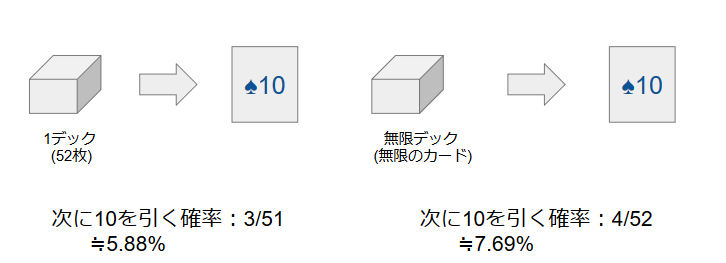
\includegraphics[width=0.7\linewidth]{./figure/DeckDiff.PNG}
 \caption{デック数による勝率の違い \label{hogehoge}}
\end{center}
\end{figure}

\bunseki{※尾崎拓海}
\section{ブラックジャックシミュレータ}
ブラックジャックのシミュレータをプログラミング言語(Python3)を用いて作成した。このシミュレータを使用して、ベーシックストラテジー、ベーシックストラテジー改変1、ベーシックストラテジー改変2、15以上になるまでヒットする戦略、16以上になるまでヒットする戦略、17以上になるまでヒットする戦略、18以上になるまでヒットする戦略のそれぞれについて勝利回数、敗北回数、引き分けた回数の3つを調べた。また、ブラックジャックを行った際の資金の推移や勝率の推移といったものを調査するためにシミュレータに所持金の概念を導入したり、実際の人間のように戦略を間違えるという処理を追加し、ダブルダウンやスプリット、サレンダーといったプレイヤー側の選択肢を追加した。このシミュレータを使用して様々な実験を実施した。ここではシミュレータ内部の詳細について記述していく。
\bunseki{※尾崎拓海}

\subsubsection{基本設計}
まず初めに、シミュレータの基本設計について説明する。今回作成したシミュレータではブラックジャックを行う際に必要となる要素をクラスとして表現した。具体的にはトランプのカードを表現するカードクラスとそれを一纏めにするデッククラス、ゲーム参加者を表すクラスとそれを継承したプレイヤークラスとディーラークラス、ゲームの勝敗を判定するマネージャークラスのそれぞれを定義した。これらのクラスを用いてブラックジャックのゲームを再現し、ベーシックストラテジーとその他の戦略を実行するプログラムを作成した。次に各クラスの詳細を記述していく。
\bunseki{※尾崎拓海}

\subsubsection{トランプのカードを表現するクラス}
このクラスでは実際のトランプのカードを表現するためにrankという変数にA~Kというトランプのランクを、suitという変数にスペード、ハート、ダイヤ、クラブのスートを定義した。また、J,Q,K,Aの絵札カードは10や11と数える必要があったので、ランクを数字に変換する処理もこのクラスに書き、valueという変数に入力した。
\bunseki{※尾崎拓海}

\subsubsection{デックを表現するクラス}
このクラスでは先程定義したカードクラスを利用してデックを定義した。具体的には先程のカードクラスの配列を作成し、その中にジョーカーを除く52種類のトランプカードを作成した。このクラスの初期化時に使用するデックの数を指定する。また、デックのシャッフルには独自に作成した関数を使用した。このシャッフル関数はPython3のrandom関数を用いて独自に設計したものであり、引数にシャッフルを行う回数を指定する。カードの配列の長さが仮に52だった場合には、1~26番目のカードからランダムに取り出したカードと、27~52番目のからランダムに取り出したカードを交換するという処理を(デック数×指定されたシャッフル回数)繰り返すという処理でシャッフル関数を作成した。
\bunseki{※尾崎拓海}

\subsubsection{ゲーム参加者を表すスーパークラス}
このクラスでは自身の手札とその手札の合計値、手札に含まれるAの枚数、バーストしているかどうかのフラグ、手札がブラックジャックとなっているかどうかのフラグのそれぞれを定義している。手札に含まれるAの枚数は自身の手札の合計値を計算する時と、ブラックジャックの条件を満たしているかどうかを判別する際に使用した。また手札の合計値を返す関数を定義し、その内側で自身がバーストしているかどうかの判定も行っている。
\bunseki{※尾崎拓海}

\subsubsection{プレイヤークラス}
このクラスは先のゲーム参加者を表すスーパークラスを継承しており、ゲームに参加しているプレイヤーを表現している。プレイヤークラスでは新たに自身の名前を表す変数と自身の勝利回数、敗北回数を記録する変数を定義した。またこのクラスでは新しく、カードを受け取る関数とヒットを行う関数、スタンドを行う関数、勝利回数と敗北回数を増加させる関数を作成した。また、ヒット、スタンド、ダブルダウン、サレンダーの処理を行う関数を作成した。
\bunseki{※尾崎拓海}

\subsubsection{ディーラークラス}
このクラスは先のゲーム参加者を表すスーパークラスを継承しており、ゲームのディーラーを表現しているクラスとなっている。ディーラークラスの中でデックをインスタンス化してディーラー側がデックを所持している事を表
現している。このクラスでは新しく、デックのシャッフル回数という変数を定義した。また、このクラスではカードを配る関数、ディーラーの手札合計が17を超えるまでカードを引き続ける関数を作成した。カードを配る関数についてはデック数有限の時とデック数無限の時とで処理を変更している。また、カウンティングを行う際に使用されたカードを数える必要があったので、使用されたカードに対応してカウントを増減させる処理をカウンティング手法ごとに記述した。
\bunseki{※尾崎拓海}

\subsubsection{ゲームマネージャークラス}
このクラスは主にゲームの勝敗判定に使用している。プレイヤーとディーラーの手札の合計値を比較し勝敗を判定する関数と、手札がブラックジャックになっているかどうかを判定する関数を作成した。また、プレイヤーの勝敗に応じて資金を移動させる処理を記述した。勝敗判定のタイミングでプレイヤーの勝利回数、敗北回数のそれぞれを記録している。
\bunseki{※尾崎拓海}

\subsubsection{メイン関数}
以上のクラスを用いてメイン関数にブラックジャックのゲームを記述した。以下にプログラムの実行手順を示す。
\begin{enumerate}
    \item ゲームに参加するプレイヤーを作成。今回はプレイヤーを一人のみ作成した。
    \item ディーラーを作成。
    \item カットカードを定義。カットカードを挟む位置はデックの半分の位置とした。
    \item ゲーム全体の実行回数を定義。今回は10万回とした。
    \item プレイヤーの戦略を配列形式で定義した。
    \item ゲームを繰り返すwhile文を作成し、ループ回数を10万回とした。
    \begin{enumerate}
        \item デックからカットカードが出てきたかを確認する。もし出てきていればデックをシャッフルする。
	  \item ディーラーが自身を含む各プレイヤーに初期カードを配る。
	  \item プレイヤーは自身の戦略に応じて掛け金を決定する。
	  \item プレイヤーは自身の戦略に沿った行動を選択する。
	  \item プレイヤーは戦略ごとに一定の確率で間違えた行動を選択する。
	  \item すべてのプレイヤーの行動が終了したことを確認後にディーラーが行動を開始する。
	  \item ディーラーの行動終了後に、勝敗判定を行う。
    \end{enumerate}
\end{enumerate}
\bunseki{※尾崎拓海}

\subsubsection{エラー時の行動}
戦略の複雑性に応じてエラーのしやすさを定義した。エラーした際の行動は以下のようになる。
\begin{itemize}
    \item ヒットとスタンドのみで構成された戦略の場合
  \begin{itemize}
        \item ヒットでエラー:スタンド
        \item スタンドでエラー:ヒット
    \end{itemize}
    \item ヒット、スタンド、ダブルダウン、スプリットで構成された戦略の場合
    \begin{itemize}
        \item ヒットでエラー:80%スタンド、20%ダブルダウン
        \item スタンドでエラー:80%ヒット、20%ダブルダウン
        \item ダブルダウンでエラー:50%ヒット、50%スタンド
        \item スプリットでエラー:スプリットを行わない
    \end{itemize}
\end{itemize}
\bunseki{※尾崎拓海}